\documentclass[a4paper]{article}

\usepackage[final]{pdfpages}
\usepackage{wrapfig}
\usepackage{subfigure}
\usepackage[letterpaper, portrait, margin=1.5in]{geometry}
\usepackage{float}
\usepackage{caption}


\captionsetup{
	font=footnotesize,
	justification=raggedright,
	singlelinecheck=false
}

\title{Polar Metabolomics Extraction}
\author{Prof. Dr. Moaraj Hasan}
\date{Jan 17th 2017}

\begin{document}

\maketitle

\section{Introduction}

\section{Data Conditioning}

All samples were run with two technical replicates which were monitored on the LC to ensure robust and reproducible spraying. High sodium and low total volumes in some samples yiled inconsistance chromatograms but the majority of samples were seen to be robust. In the electrospray 19 000 featured were detected, 4000 of which could be annotated with some certainty, the majority of which however remains complex high molecular weight material.  

\begin{figure}[h]
	\centering
	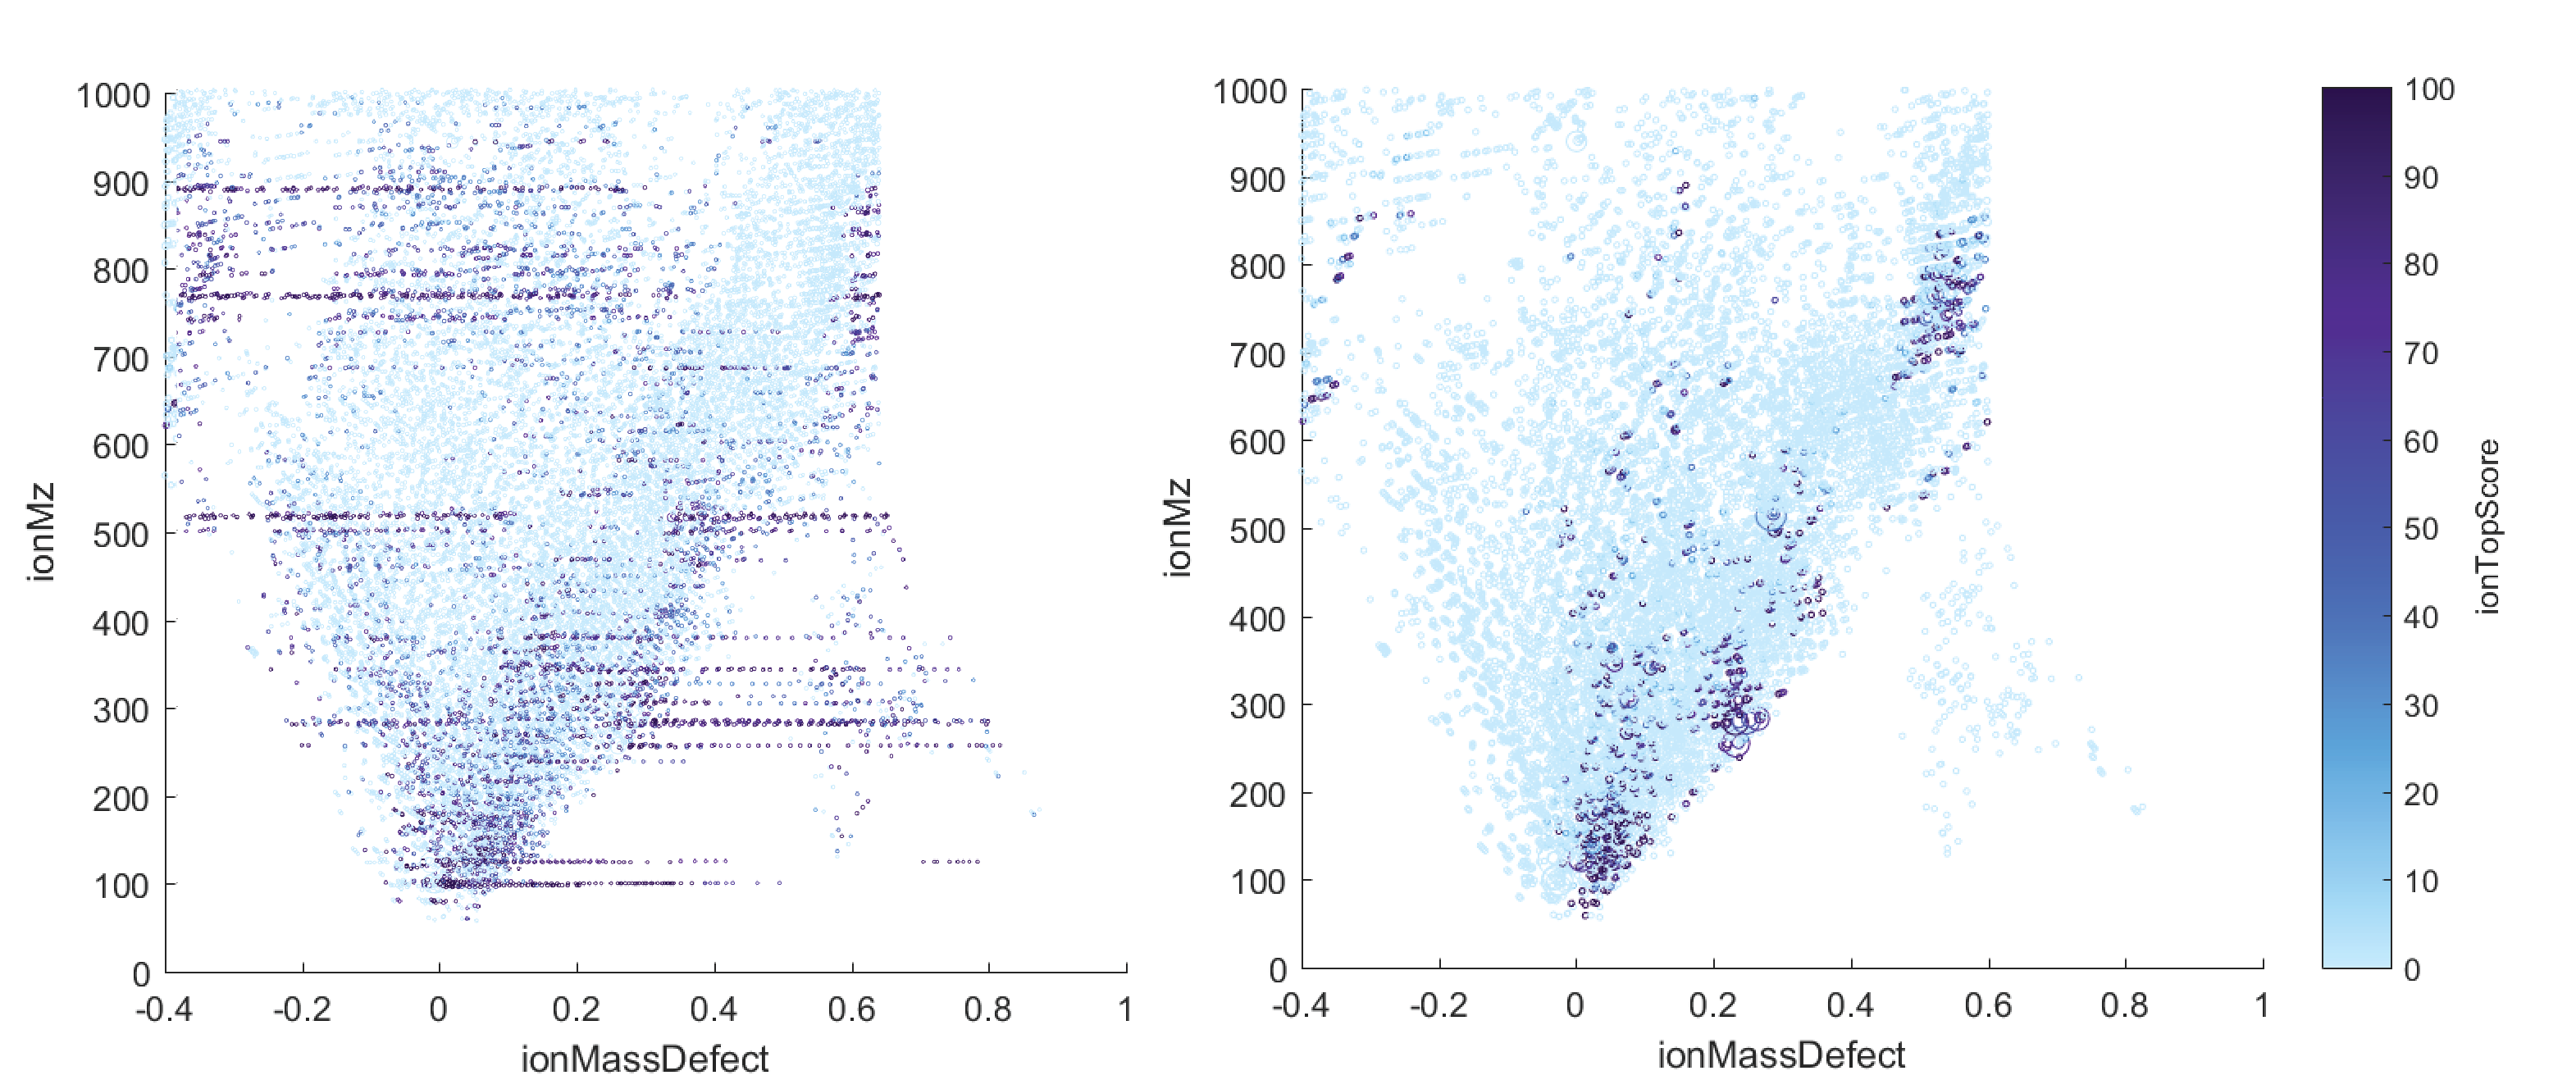
\includegraphics[width=1.0\linewidth]{Peak_filtering}
	\caption{Left: All annotated peak annotated automatically \newline
		Right: Ringing Peaks and impossible mass combinations filtered}
	\label{fig:peakfiltering}
\end{figure}

During analog to digital signal conversion detector and preamplifier electronic noise is recorded and appears in the data, as does any ugliness in the pulse shape. Absolute quantification is very difficult because the detector gain has a first order effect on spectrum peak heights. Detector analogue gain is a highly non-linear function of excitation voltage, subject to drift and difficult to measure unless extra hardware is present, such as a Faraday cup. In practice an internal standard is necessary (a mass peak to normalise against). In these metabolic study no house keeping metabolites are availible for normalization nor are the samples spiked with an internal standard, as a results relative signal intensities are compared that than absolute counts. 


\section{Extraction Conditions}

Four extraction conditions were tested to determine the optimal extraction efficiency and robust metabolic converage. 
In a hot extraction, timing must be kept meticulously, in order to minize degredation and restarting metabolic reactions.
A homogenization step is included in the protocol to lyse cells as the buffer unsufficently micelle disrupting to dissolve cellular membrane. 
After homogenization, the hot bath is meant fo denature enyzmes that increase the extraciton rate.
LIke wise in the cold extraction [40:40:20] MeOH, ACN and H2O extraction mixture is meant to solubilize cells and poison enzymes.
Two cold extactions times were used , 1hours and 24 hours at -20C to determine the extraction kinetics and optimal extrcation times.
We also attempted a 24 hour cold extraction without the homogenizatin step as it can introduce impurities and cross samples contaminents if the homogenization head is not properly cleaned. 
Morever, the homogenization step adds a minute to each protocol and adds timing complication into the proctol, 
warranting us to determine if it can be circumvented.

\subsection{Warm Extraction}
In the warm samples extraction protocol, samples are kept at -20°C, weighed in cell culture tubes to allow for the homogenization head to read the bottom of the plate.
They are homogenized to lyse cells, at which point vicous heating from the homogenizer brings the sample temperature up quite quickly. It is for this reason they must rapidly be transferred into
a 75°C bath to prevent

\begin{figure}[h]
	\centering
	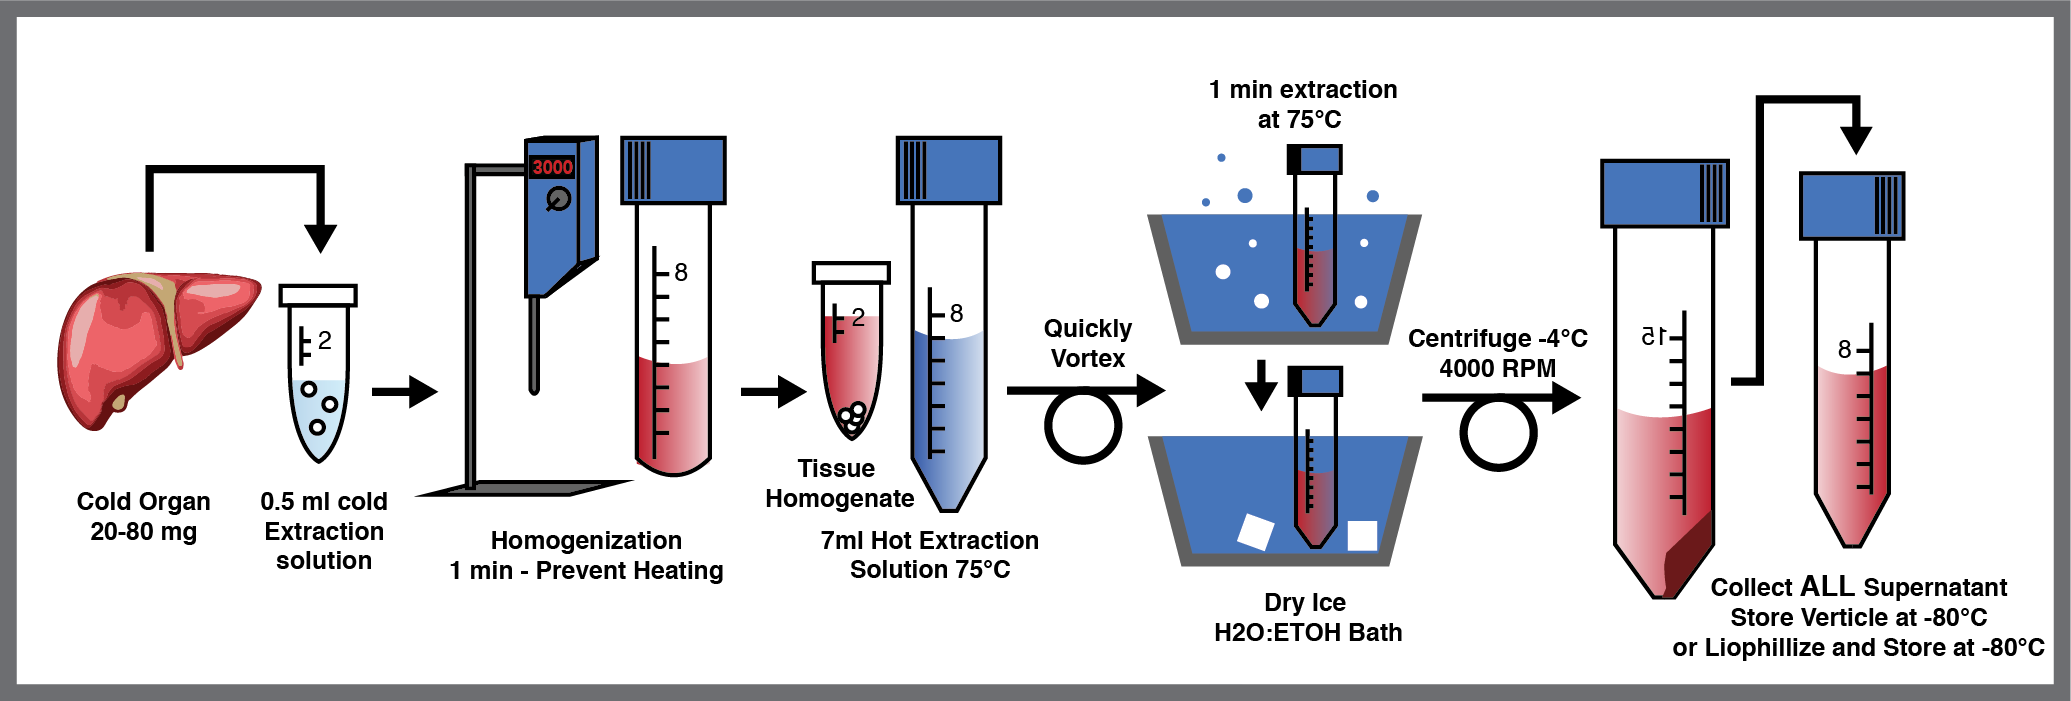
\includegraphics[width=1\linewidth]{Metab-Proto-MH-20170120-3}
	\caption{Hot Polar Metabolite Extraction Protocol}
	\label{fig:metab-proto-mh-20170105}
\end{figure}

\subsection{Cold Extraction}

The cold extraciton protocol uses a methanol, acetonitrile and water mixture to quickly neutralize ezymes that may be active in the solution and thus allow for easier handling. Samples are kept at -20°C while prepaing and during extraction however, they are still heated during the homogenization step. 

\begin{figure}[h]
	\centering
	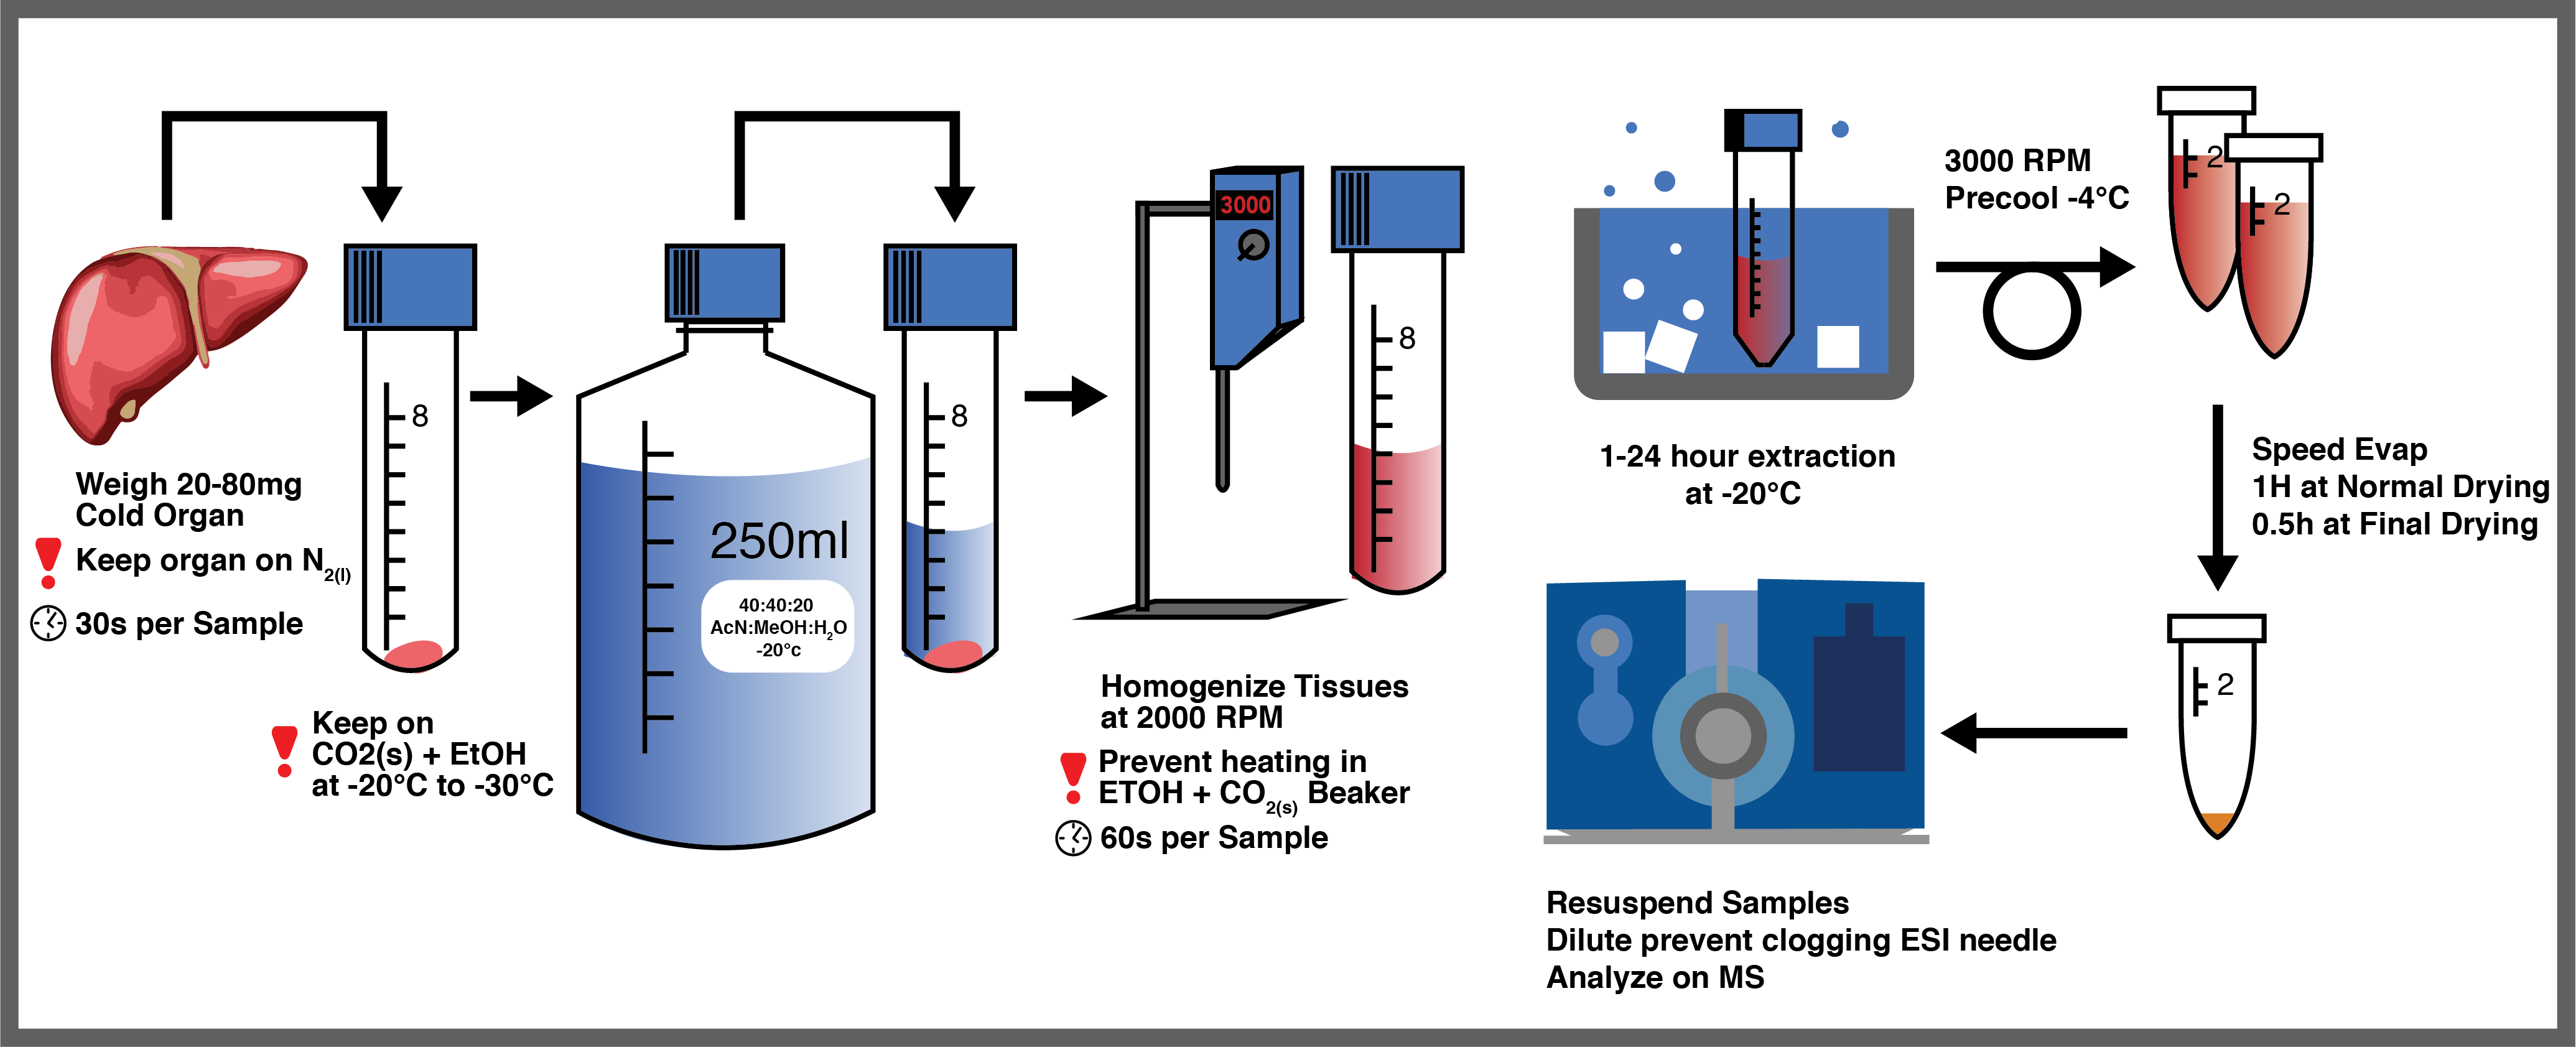
\includegraphics[width=\linewidth]{Metab-Cold-Proto-MH-20170120}
	\caption{Cold Polar Metabolite Extraction Protocol}
	\label{fig:metab-cold-proto-mh-20170105}
\end{figure}


\section{Results}


where are the adjsutsted p values and p values gernerated 


\subsection{Hot and Cold Extraction Performace}
\begin{figure}[H]
	\centering
	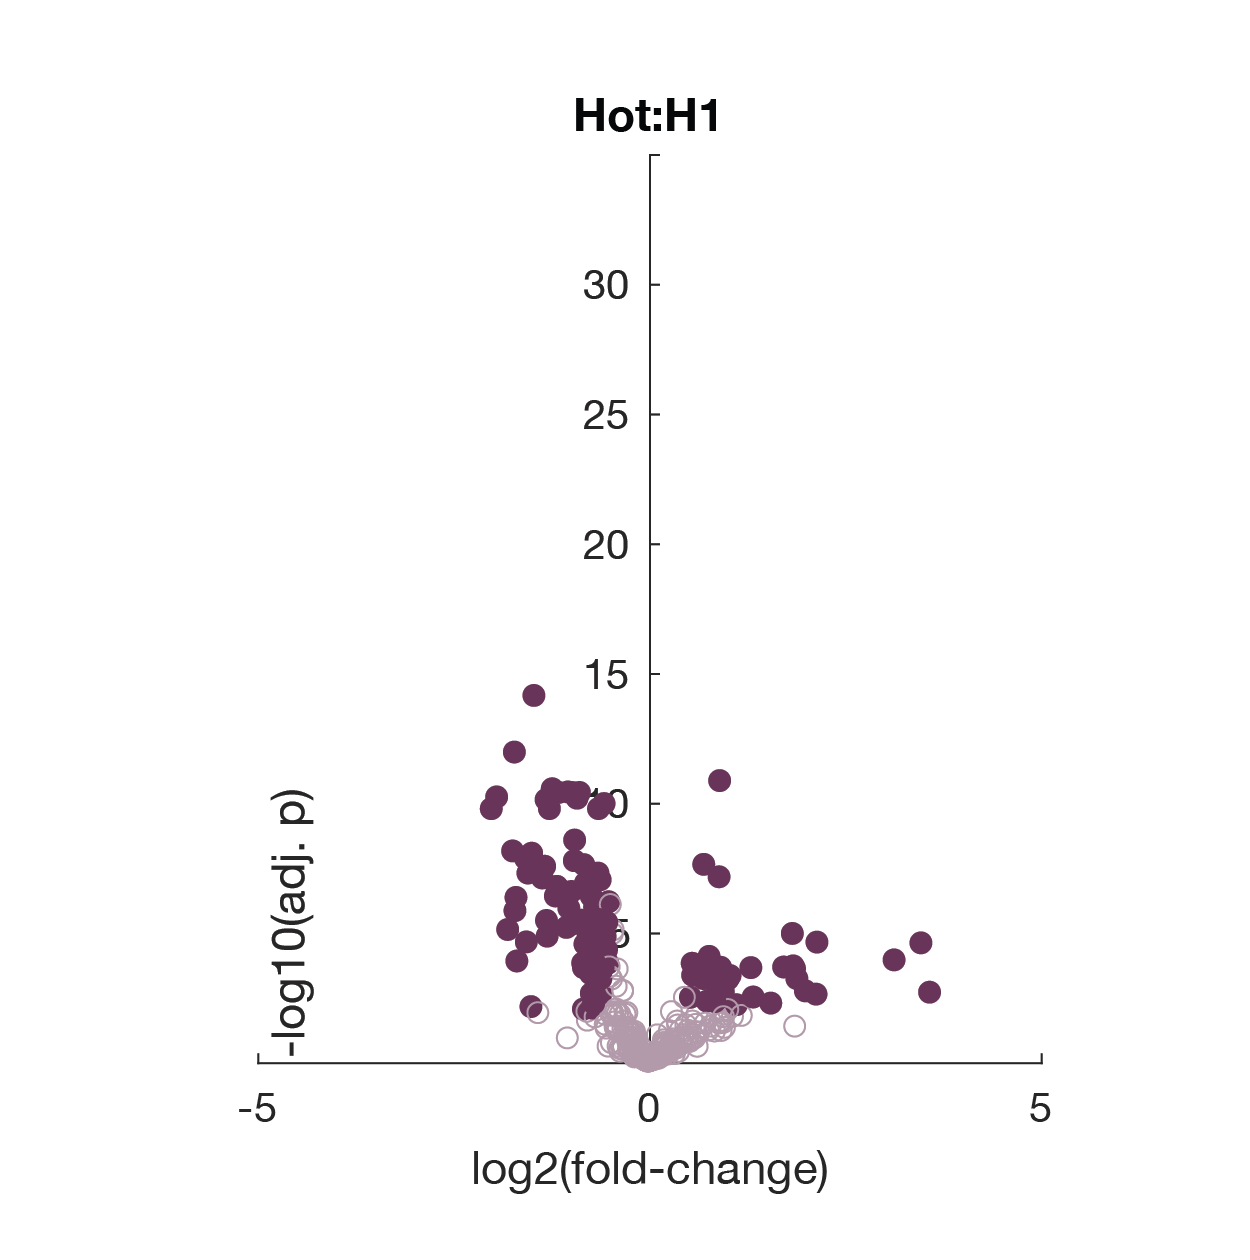
\includegraphics[width=0.5\linewidth]{Hot_H1_01}
	\caption{Volcano Plot of P-Values and Log2 Fold Chagnes seen between Hot Extraction protocol and Standard Cold Extraction Protocol}
	\label{fig:hoth101}
\end{figure}


Results indicate the homogenization is not nesceaary to sufficiently extract polar metabolites from the cells. Additionally, cold and hot extraction both perform similarly in terms of the coverage of metabolites that are extracted, however the varibation in the spectra is much larger in the cold extraction due to the longer processing times in which degredatin products accumulate. In the figure below all annoatatation are displayed on 

\subsection{Extraction Time Performace}
\begin{figure}[H]
	\centering
	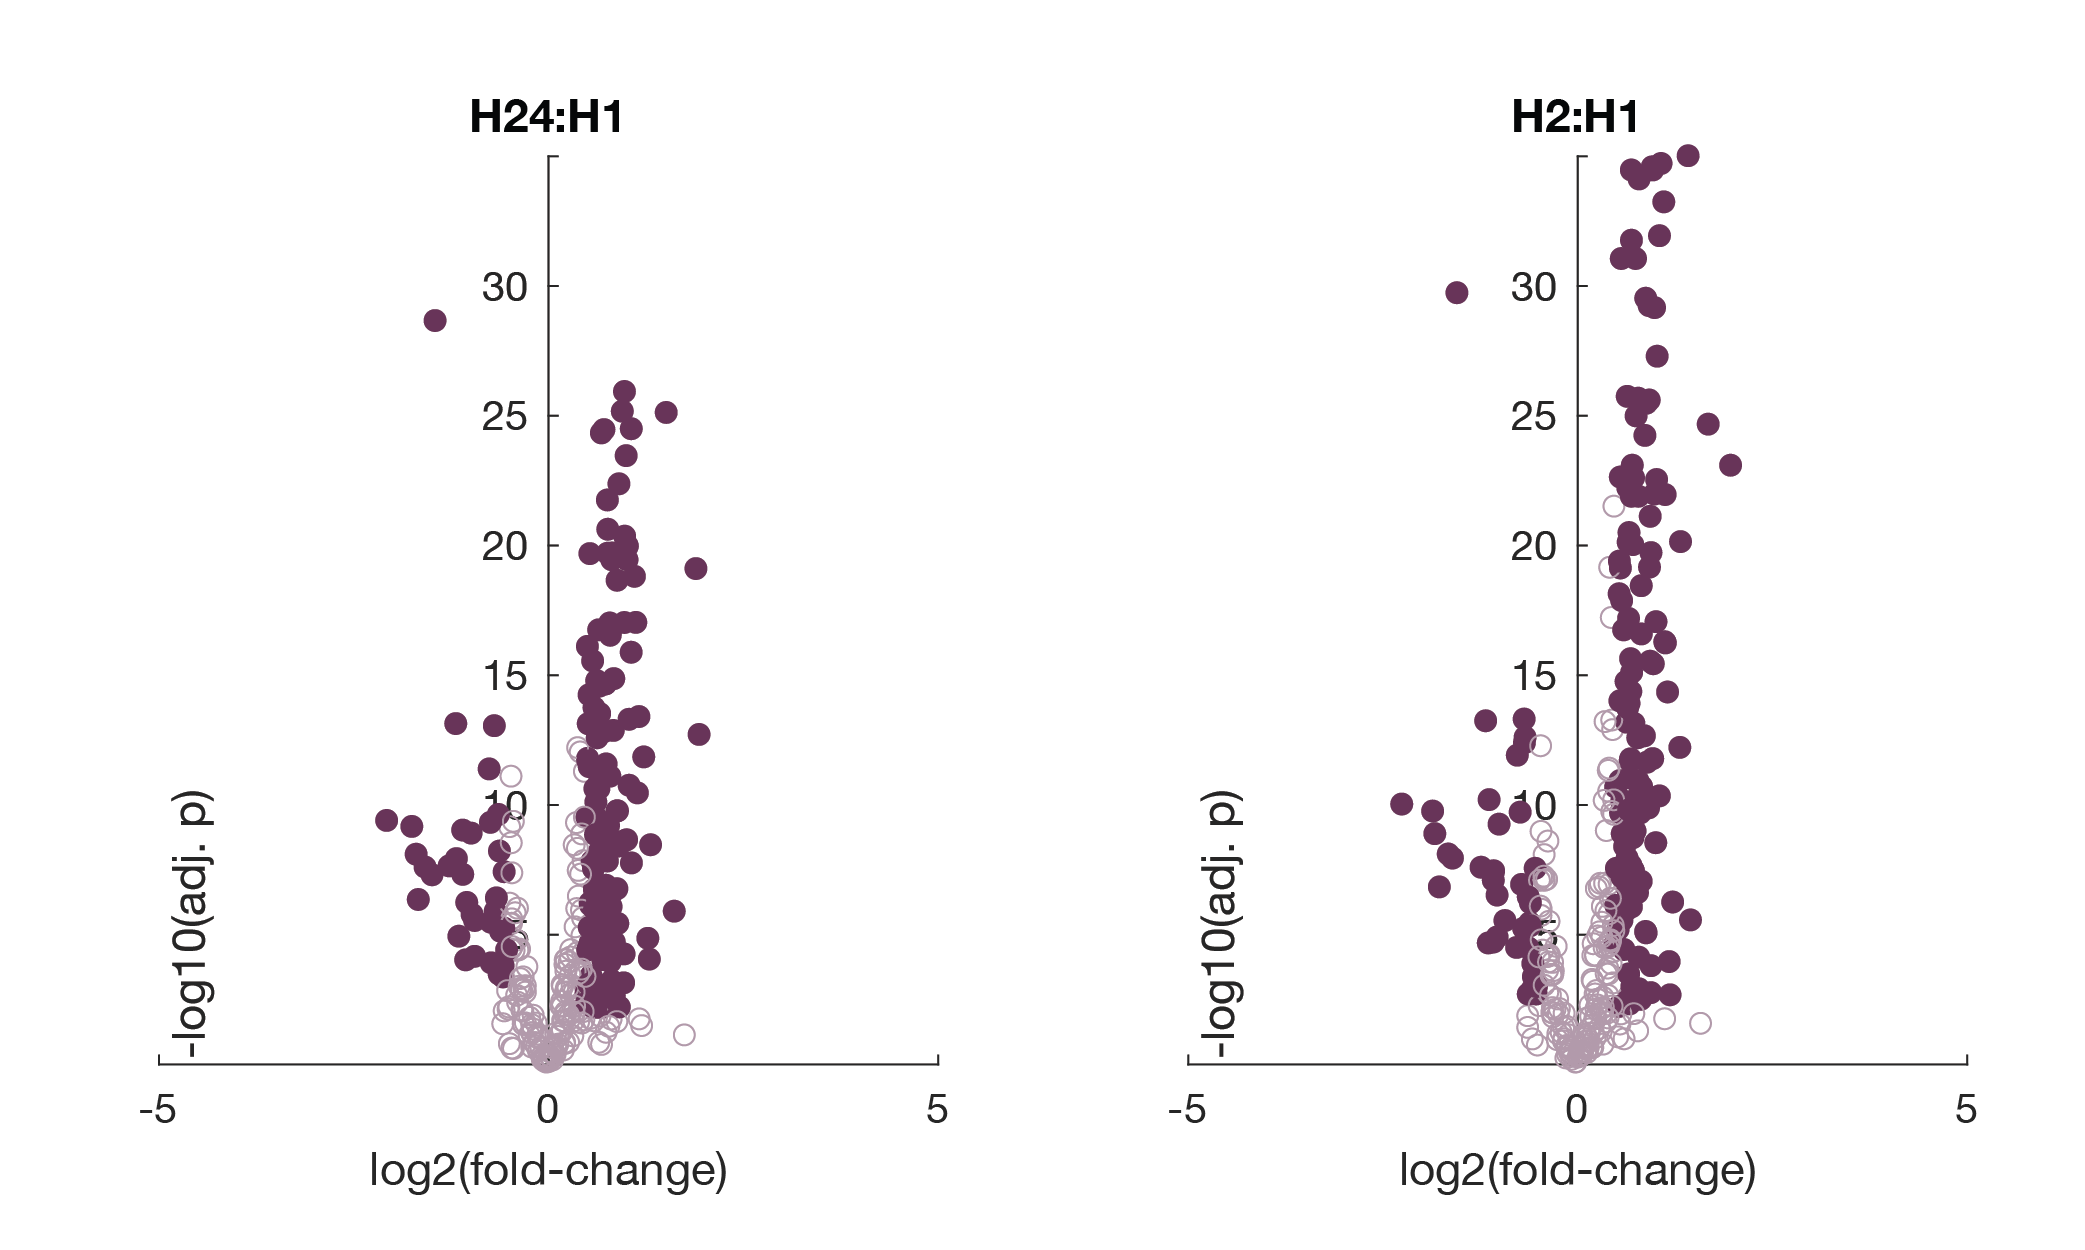
\includegraphics[width=0.7\linewidth]{H1-H24-H2-01}
	\caption{Volcano Plot of P-Values and Log2 Fold Chagnes seen between Standard Cold Extraction Protocols with an additional 1hour and 24 hour extraction perdion as compared to the standard cold extraction protocol}
	\label{fig:h1-h24-h2-01}
\end{figure}

\subsection{Effect of Homogenization on Performance}
\begin{figure}[H]
	\centering
	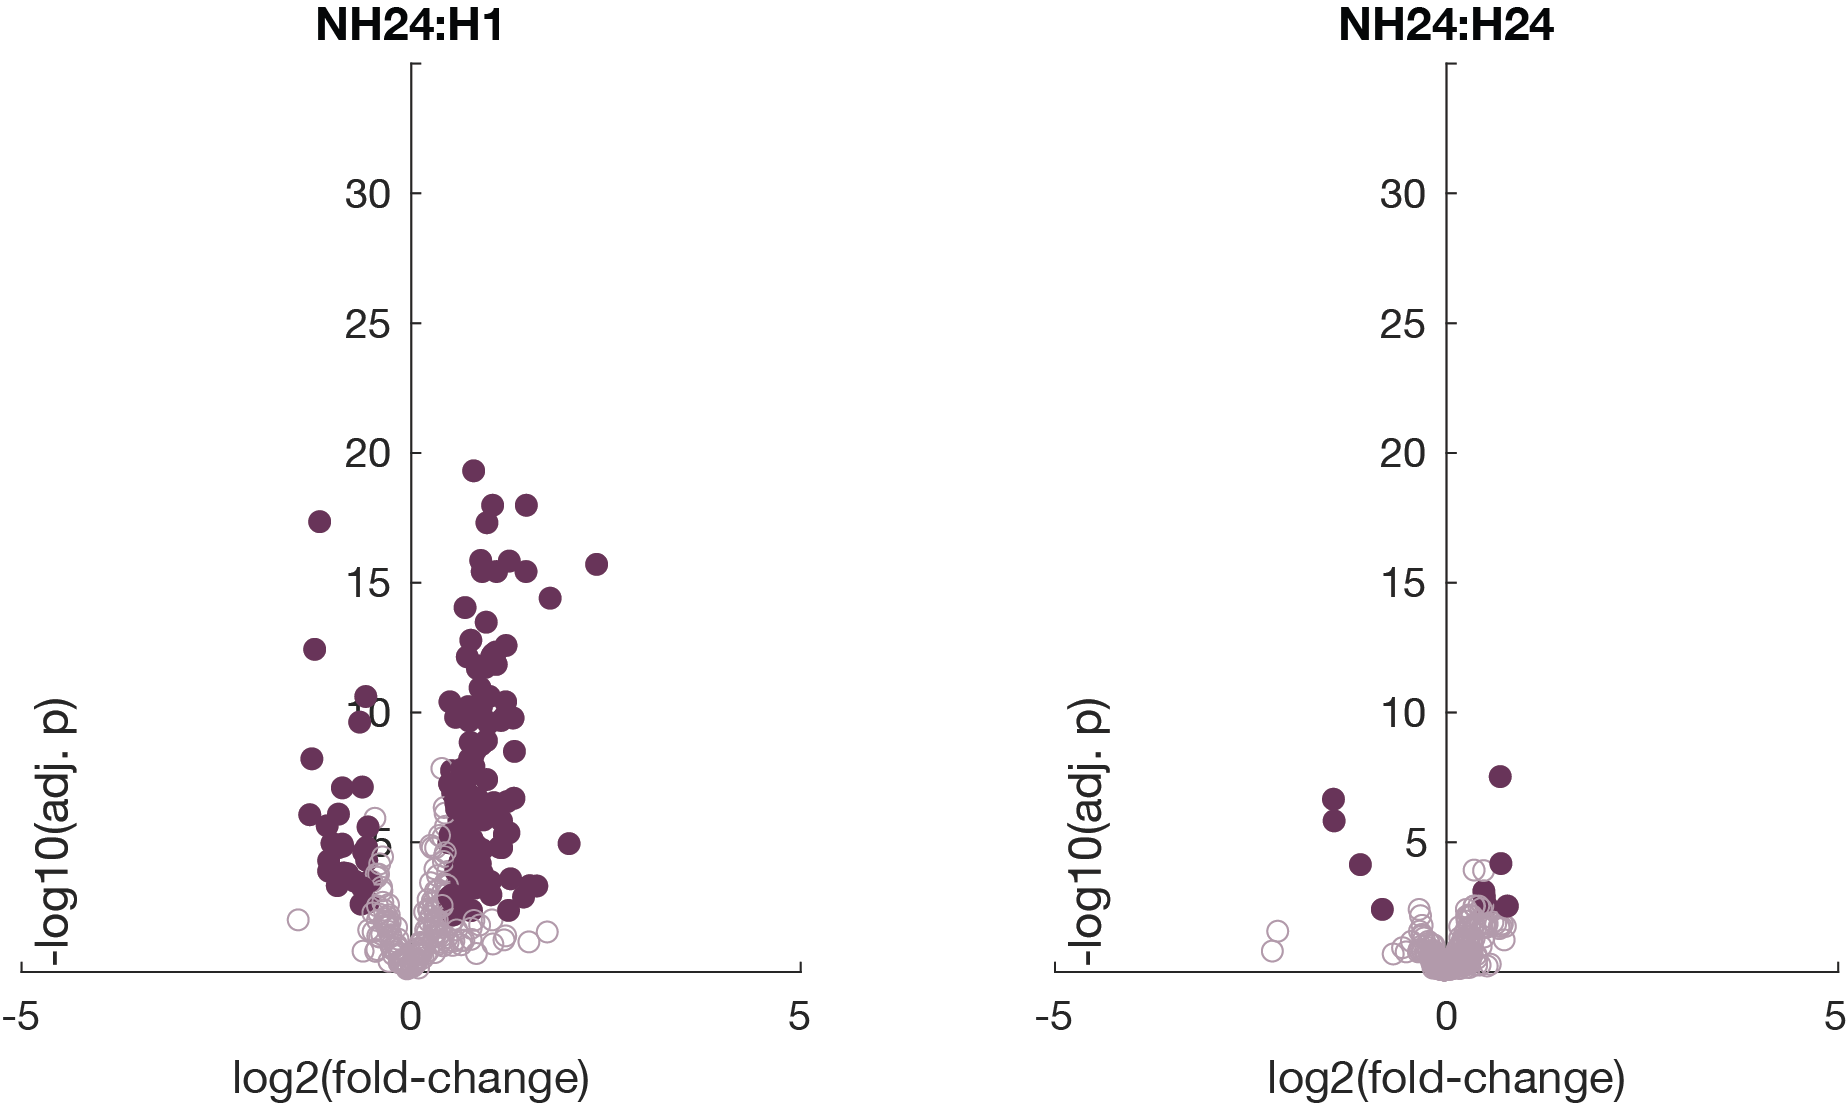
\includegraphics[width=0.7\linewidth]{NH24}
	\caption{Volcano Plot of P-Values and Log2 Fold Chagnes seen between Standard Cold Extraction Protocols with an additional 1hour and 24 hour extraction perdion as compared to the standard cold extraction protocol}
	\label{fig:nh24}
\end{figure}



\section{Discussion}
\subsection{Components of Chow and High Fat diet}
Regular chow is composed of agricultural byproducts, such as ground wheat, corn, or oats, alfalfa and soybean meals, a protein source such as fish, and vegetable oil and is supplemented with minerals and vitamins. Thus, chow is a high fiber diet containing complex carbohydrates, with fats from a variety of vegetable sources. Chow is inexpensive to manufacture and is palatable to rodents. In contrast, defined high-fat diets consist of amino acid supplemented casein, cornstarch, maltodextrose or sucrose, and soybean oil or lard, also supplemented with minerals and vitamins. Fiber is often provided by cellulose. Chow and defined diets may exert significant separate and independent unintended effects on the measured phenotypes in any research protocol.

\subsection{Mouse Estrous Cycle}

In humans, the reproductive cycle, called the menstrual cycle, lasts approximately 28 days, in rodents this cycle, called the estrous cycle, lasts approximately 4-5 days. Although this short cycles make mice ideal candidates for studying chages during reproductive cycles, they also present a complicating factor in assesing sterols and cyclic metabolites in metabolomic screens. Estural cycle data is not included in the phenotypic observation of the mice and as a result cannot be reliably excluded.

\section{Appendix}

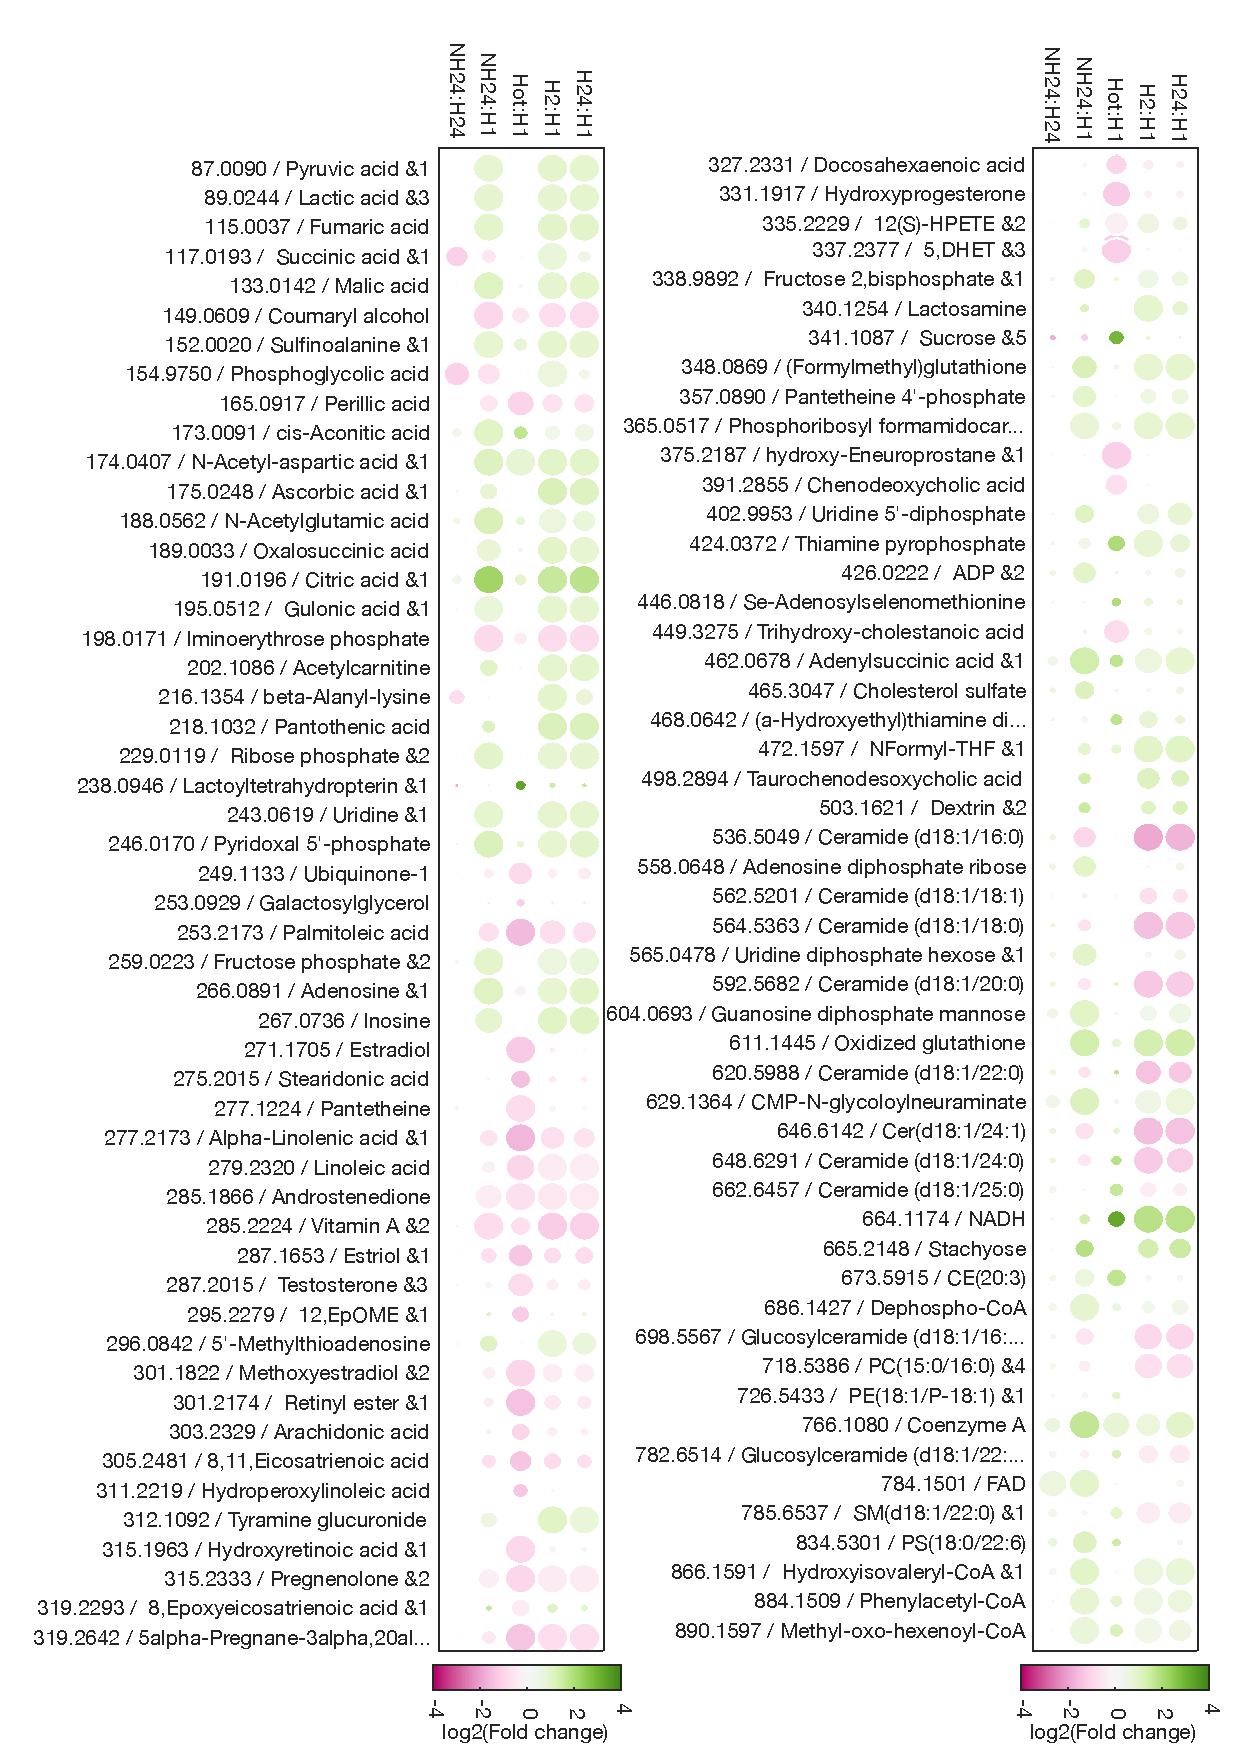
\includepdf[pages=-]{bubbles1.pdf}



\bibliographystyle{plain}
\bibliography{bibliography.bib}
\end{document}